\documentclass{beamer}

% Theme selection
\usetheme{Madrid}
\usecolortheme{beaver} % Professional red/gray color palette

% Required packages
\usepackage{amsmath, amsfonts, amssymb}
\usepackage{tikz}
\usepackage{hyperref}
\usetikzlibrary{shapes.geometric, positioning}

% =======================================================
% Presentation Details (Title / Front Page Setup)
% =======================================================
\title[Discrete Mathematics]{Set Theory and Posets}
\subtitle{Sets, Operations, Inclusion--Exclusion, and Hasse Diagrams}

\author[Your Name]{%
  \textbf{Author:} Jacob Ninan Raju \\[0.3em]
  \\Semester 1:M.Tech in Computer Science and Engineering with Specialization
  in Artificial Intelligence and Software Engieering
  \small 
  \\ Course: Mathematics For Computing
}

\institute[Your University]{
  Department of Computer Science \& Engineering \\
  CUSAT
}

\date{\today}

\
}

% =======================================================
% Main Document Content
% =======================================================
\begin{document}

% -------------------------------------------------------
% Title Frame (Front Page)
% -------------------------------------------------------
\begin{frame}[plain] % 'plain' option removes headers/footers for a clean front page
    \titlepage
\end{frame}

% -------------------------------------------------------
% Table of Contents
% -------------------------------------------------------
\begin{frame}{Outline}
    \tableofcontents
\end{frame}

% -------------------------------------------------------
\section{Introduction to Sets}
% -------------------------------------------------------
\begin{frame}{What is a Set?}
    \begin{definition}
        A \textbf{set} is a well-defined collection of distinct objects, referred to as elements or members of the set.
    \end{definition}

    \vspace{0.5cm}
    \textbf{Key Concepts:}
    \begin{itemize}
        \item If $x$ is an element of set $A$, we write $x \in A$.
        \item If $x$ is not an element of set $A$, we write $x \notin A$.
        \item Sets are typically denoted by capital letters ($A, B, C$), while elements are denoted by lowercase letters ($a, b, c$).
    \end{itemize}
\end{frame}

% -------------------------------------------------------
\section{Set Builder Form}
% -------------------------------------------------------
\begin{frame}{Representing Sets: Set-Builder Form}
    Sets can be described in two primary ways:
    \begin{enumerate}
        \item \textbf{Roster/Tabular Form:} Explicitly listing elements.
        \begin{itemize}
            \item Example: $A = \{2, 4, 6, 8\}$
        \end{itemize}
        \item \textbf{Set-Builder Form:} Stating the property that all elements must satisfy.
    \end{enumerate}

    \vspace{0.3cm}
    \begin{block}{General Notation}
        \[ S = \{ x \mid P(x) \} \quad \text{or} \quad S = \{ x : P(x) \} \]
        \small{Read as: ``The set of all $x$ such that $P(x)$ is true.''}
    \end{block}

    \textbf{Examples:}
    \begin{itemize}
        \item $E = \{ x \in \mathbb{Z} \mid x \text{ is even and } 0 < x < 10 \}$
        \item $B = \{ x \in \mathbb{R} \mid x^2 - 4 = 0 \}$ (which equals $\{-2, 2\}$)
    \end{itemize}
\end{frame}

% -------------------------------------------------------
\section{Types of Sets}
% -------------------------------------------------------
\begin{frame}{Common Types of Sets}
    \begin{itemize}
        \item \textbf{Empty (Null) Set ($\emptyset$ or $\{\}$):} A set containing no elements.
        \item \textbf{Singleton Set:} A set containing exactly one element, e.g., $\{5\}$.
        \item \textbf{Finite Set:} A set with a countable number of elements, e.g., $A = \{a, b, c\}$.
        \item \textbf{Infinite Set:} A set with infinitely many elements, e.g., $\mathbb{N} = \{1, 2, 3, \dots\}$.
        \item \textbf{Universal Set ($U$):} The set containing all possible objects under consideration.
        \item \textbf{Subset ($A \subseteq B$):} Every element of $A$ is also an element of $B$.
        \item \textbf{Power Set ($\mathcal{P}(A)$):} The set of all subsets of $A$.
        \begin{itemize}
            \item If $|A| = n$, then $|\mathcal{P}(A)| = 2^n$.
        \end{itemize}
    \end{itemize}
\end{frame}

% -------------------------------------------------------
\section{Set Operations}
% -------------------------------------------------------
\begin{frame}{Fundamental Set Operations}
    \begin{block}{Union ($A \cup B$)}
        $A \cup B = \{ x \mid x \in A \text{ or } x \in B \}$
    \end{block}

    \begin{block}{Intersection ($A \cap B$)}
        $A \cap B = \{ x \mid x \in A \text{ and } x \in B \}$
    \end{block}

    \begin{block}{Difference ($A \setminus B$ or $A - B$)}
        $A \setminus B = \{ x \mid x \in A \text{ and } x \notin B \}$
    \end{block}

    \begin{block}{Complement ($A^c$ or $A'$)}
        $A^c = U \setminus A = \{ x \in U \mid x \notin A \}$
    \end{block}
\end{frame}

\begin{frame}{Venn Diagrams: Union \& Intersection}
    \begin{figure}[h]
        \centering
        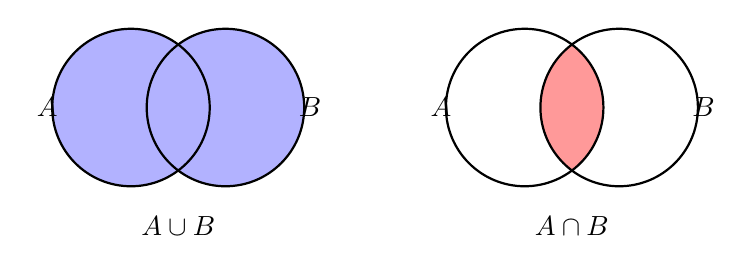
\begin{tikzpicture}
            % Union Diagram
            \begin{scope}[shift={(-2.5,0)}]
                \fill[blue!30] (0,0) circle (1cm);
                \fill[blue!30] (1.2,0) circle (1cm);
                \draw[thick] (0,0) circle (1cm) node[left=0.8cm] {$A$};
                \draw[thick] (1.2,0) circle (1cm) node[right=0.8cm] {$B$};
                \node at (0.6,-1.5) {$A \cup B$};
            \end{scope}

            % Intersection Diagram
            \begin{scope}[shift={(2.5,0)}]
                \begin{scope}
                    \clip (0,0) circle (1cm);
                    \fill[red!40] (1.2,0) circle (1cm);
                \end{scope}
                \draw[thick] (0,0) circle (1cm) node[left=0.8cm] {$A$};
                \draw[thick] (1.2,0) circle (1cm) node[right=0.8cm] {$B$};
                \node at (0.6,-1.5) {$A \cap B$};
            \end{scope}
        \end{tikzpicture}
    \end{figure}
\end{frame}

% -------------------------------------------------------
\section{Inclusion--Exclusion Principle}
% -------------------------------------------------------
\begin{frame}{Inclusion--Exclusion Principle (PIE)}
    The Inclusion--Exclusion Principle helps compute the cardinality of the union of multiple sets by accounting for overlapping elements.

    \vspace{0.3cm}
    \begin{alertblock}{For Two Sets}
        \[ |A \cup B| = |A| + |B| - |A \cap B| \]
    \end{alertblock}

    \vspace{0.3cm}
    \begin{alertblock}{For Three Sets}
        \[
        |A \cup B \cup C| = |A| + |B| + |C| - |A \cap B| - |B \cap C| - |A \cap C| + |A \cap B \cap C|
        \]
    \end{alertblock}
\end{frame}

\begin{frame}{PIE Example}
    \textbf{Problem:} In a class of 50 students, 30 play Football, 25 play Basketball, and 10 play both. How many students play at least one game?

    \vspace{0.4cm}
    \textbf{Solution:}
    Let $F$ be the set of Football players and $B$ be the set of Basketball players.
    \begin{itemize}
        \item $|F| = 30$
        \item $|B| = 25$
        \item $|F \cap B| = 10$
    \end{itemize}

    \[
    |F \cup B| = |F| + |B| - |F \cap B|
    \]
    \[
    |F \cup B| = 30 + 25 - 10 = 45
    \]

    \textbf{Answer:} 45 students play at least one game.
\end{frame}

% -------------------------------------------------------
\section{Hasse Diagrams}
% -------------------------------------------------------
\begin{frame}{Posets and Hasse Diagrams}
    \begin{definition}
        A \textbf{Partially Ordered Set (Poset)} is a pair $(S, \le)$ where $S$ is a set and $\le$ is a binary relation that is \textit{reflexive}, \textit{antisymmetric}, and \textit{transitive}.
    \end{definition}

    \vspace{0.3cm}
    \textbf{What is a Hasse Diagram?}
    \begin{itemize}
        \item A simplified visual representation of a finite poset.
        \item \textbf{Rules for construction:}
        \begin{enumerate}
            \item Omit self-loops (implied by reflexivity).
            \item Omit transitive edges (e.g., if $a \le b$ and $b \le c$, do not draw $a \to c$).
            \item Draw edges without directional arrows; place larger elements higher up.
        \end{enumerate}
    \end{itemize}
\end{frame}

\begin{frame}{Hasse Diagram Example}
    \textbf{Example:} Hasse Diagram for the divisibility relation on $D_{12} = \{1, 2, 3, 4, 6, 12\}$.

    \begin{figure}[h]
        \centering
        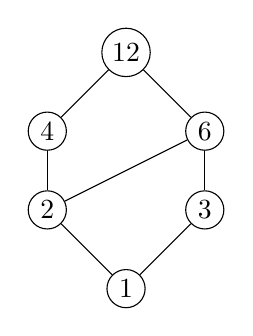
\begin{tikzpicture}[node distance=1.2cm and 1.5cm, every node/.style={circle, draw, inner sep=2pt}]
            % Nodes
            \node (12) at (0, 3) {12};
            \node (4) at (-1, 2) {4};
            \node (6) at (1, 2) {6};
            \node (2) at (-1, 1) {2};
            \node (3) at (1, 1) {3};
            \node (1) at (0, 0) {1};

            % Edges
            \draw (1) -- (2);
            \draw (1) -- (3);
            \draw (2) -- (4);
            \draw (2) -- (6);
            \draw (3) -- (6);
            \draw (4) -- (12);
            \draw (6) -- (12);
        \end{tikzpicture}
    \end{figure}
\end{frame}

% -------------------------------------------------------
% Conclusion Slide
% -------------------------------------------------------
\begin{frame}
    \centering
    \Huge \textbf{Thank You!} \\
    \vspace{0.5cm}
    \Large 
\end{frame}

\end{document}

